\documentclass[12pt]{article}
\usepackage[a4paper, margin=1in]{geometry}
\usepackage{amsmath}
\usepackage{graphicx}
\usepackage{hyperref}
\usepackage{times}
\usepackage{listings}
\usepackage{xcolor}  % For colored syntax highlighting
\usepackage{graphicx}
\usepackage{subcaption}


% Code listing style
\definecolor{codegreen}{rgb}{0,0.6,0}
\definecolor{codegray}{rgb}{0.5,0.5,0.5}
\definecolor{codepurple}{rgb}{0.58,0,0.82}
\definecolor{backcolour}{rgb}{0.95,0.95,0.92}

\lstdefinestyle{mystyle}{
    backgroundcolor=\color{backcolour},   
    commentstyle=\color{codegreen},
    keywordstyle=\color{magenta},
    numberstyle=\tiny\color{codegray},
    stringstyle=\color{codepurple},
    basicstyle=\ttfamily\footnotesize,
    breakatwhitespace=false,         
    breaklines=true,                 
    captionpos=b,                    
    keepspaces=true,                 
    numbers=left,                    
    numbersep=5pt,                  
    showspaces=false,                
    showstringspaces=false,
    showtabs=false,                  
    tabsize=2
}

\lstset{
  language=Python,
  backgroundcolor=\color{backcolour},
  commentstyle=\color{codegreen},
  keywordstyle=\color{magenta},
  numberstyle=\color{codegray},
  stringstyle=\color{codepurple},
  basicstyle=\ttfamily\footnotesize,
  breaklines=true,
  captionpos=b,
  keepspaces=true,
  numbers=left,
  numbersep=5pt,
  showspaces=false,
  showstringspaces=false,
  showtabs=false,
  tabsize=2
}


\lstset{style=mystyle}

\title{Assignment 2}
\author{Cadei Paolo \\ Student Number: 14060876}
\date{31 May 2025}

\begin{document}
\maketitle

\section{Question}

\begin{lstlisting}
import random
import numpy as np
from queue import PriorityQueue

def update_Q(gridworld, Q, s, a, s_prime, r, alpha=0.1, gamma=0.95):
    a_idx = gridworld.actions_to_idx[a]
    return Q[s, a_idx] + alpha * (r + gamma * np.max(Q[s_prime]) - Q[s, a_idx])

def greedy_policy(gridworld, Q):
    policy = np.zeros_like(Q)
    states_, actions_ = np.nonzero((Q.T == np.max(Q, axis=1)).T)
    for s in np.arange(gridworld.nstates):
        policy[s, np.random.choice(actions_[states_ == s])] = 1.0
    return policy

def train_prioritized_sweeping(gridworld, episodes=10, n=5, alpha=0.1, gamma=0.95, epsilon=0.1, theta=1e-5):

    Q = src.initialize_Q(gridworld, random=False)
    model = {}
    steps_history = np.array([], dtype=int)
    priority_queue = PriorityQueue()
    predecessors = {}
    
    for ep in range(episodes):

        s = gridworld.initial_state
        steps = 0

        while not s == gridworld.terminal_state:

            steps += 1

            # Epsilon-greedy action selection
            if epsilon < np.random.rand():  # greedy
                a_idx = np.random.choice(np.nonzero(Q[s] == np.max(Q[s]))[0])
            else:  # random
                a_idx = np.random.randint(len(gridworld.actions))
            a = gridworld.actions[a_idx]

            # Environment interaction
            s_prime, r = gridworld.interact(s, a)

            # Update Interaction with Environment

            Q[s, a_idx] = update_Q(gridworld, Q, s, a, s_prime, r,  alpha=alpha, gamma=gamma)

            # Store model
            model[(s, a)] = (s_prime, r)

            # Store predecessor
            if s_prime not in predecessors:
                predecessors[s_prime] = [(s, a)]
            else:
                predecessors[s_prime].append((s, a))

            # Compute priority
            P = abs(r + gamma * np.max(Q[s_prime]) - Q[s, a_idx])
            if P > theta:
                priority_queue.put((-P, s, a))

            # Planning
            for _ in range(n):
                if priority_queue.empty():
                    break
                
                _, s_pl, a_pl = priority_queue.get()
                s_prime_pl, r_pl = model[(s_pl, a_pl)]
                a_pl_idx = gridworld.actions_to_idx[a_pl]
                Q[s_pl, a_pl_idx] = update_Q(gridworld, Q, s_pl, a_pl, s_prime_pl, r_pl, alpha=alpha, gamma=gamma)

                # Update predecessors
                for s_pred, a_pred in predecessors.get(s_pl, []):
                    _, r_pred = model[(s_pred, a_pred)]
                    a_pred_idx = gridworld.actions_to_idx[a_pred]
                    P_pred = abs(r_pred + gamma * np.max(Q[s_pl]) - Q[s_pred, a_pred_idx])
                    if P_pred > theta:
                        priority_queue.put((-P_pred, s_pred, a_pred))

            # Move to next state
            s = s_prime

        steps_history = np.append(steps_history, steps)

    return Q, steps_history, greedy_policy(gridworld, Q)
\end{lstlisting}

\pagebreak

\noindent The comparison between Dyna-Q and Prioritized Sweeping highlights key differences in their performance, learning dynamics, and efficiency. \\

\begin{figure}[h!]
    \centering
    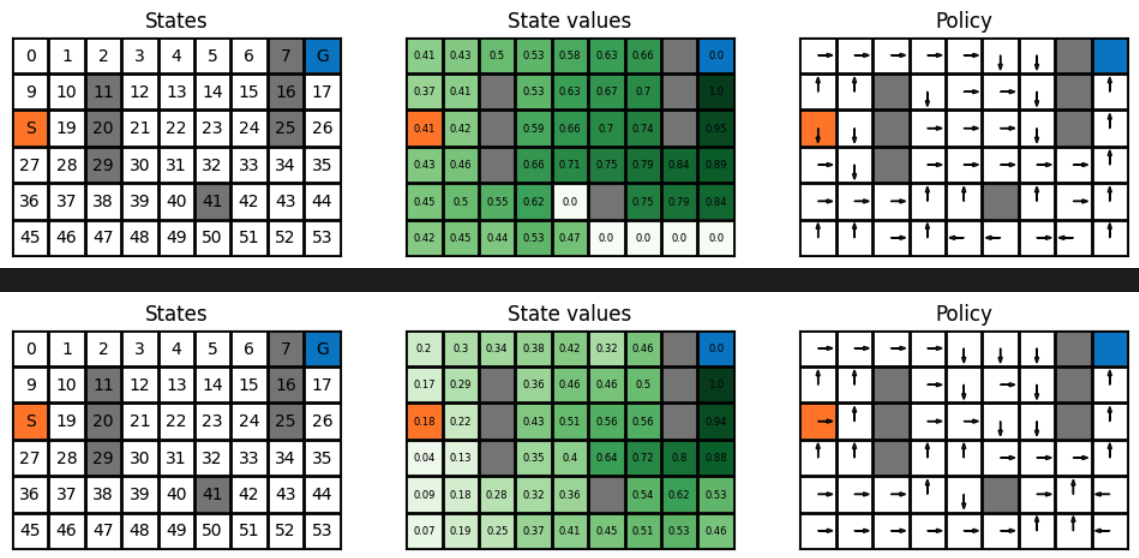
\includegraphics[width=0.8\textwidth]{Assignment2/Images/original_50_1.png}
    \caption{Visualization of state values and policy arrows in the original 6x9 Gridworld.}
    \label{fig:original_values_policy}
\end{figure}

\noindent The visualizations of state values and policies show that Prioritized Sweeping more effectively propagates values from the goal state and converges toward an optimal policy more rapidly than Dyna-Q. We can also see that Prioritised-Sweeping has a lot more non-zero values than Dyna-Q when it comes to state-values. Additionally, the policy arrows derived from Prioritized Sweeping exhibit more consistent and direct paths to the goal, indicating better exploitation of the environment’s structure, while Dyna-Q's policy appears noisier and more exploratory in the early stages.
This becomes even more accentuated if we increase the size of the Gridworld environment to 20x20. \\

\begin{figure}[h!]
    \centering
    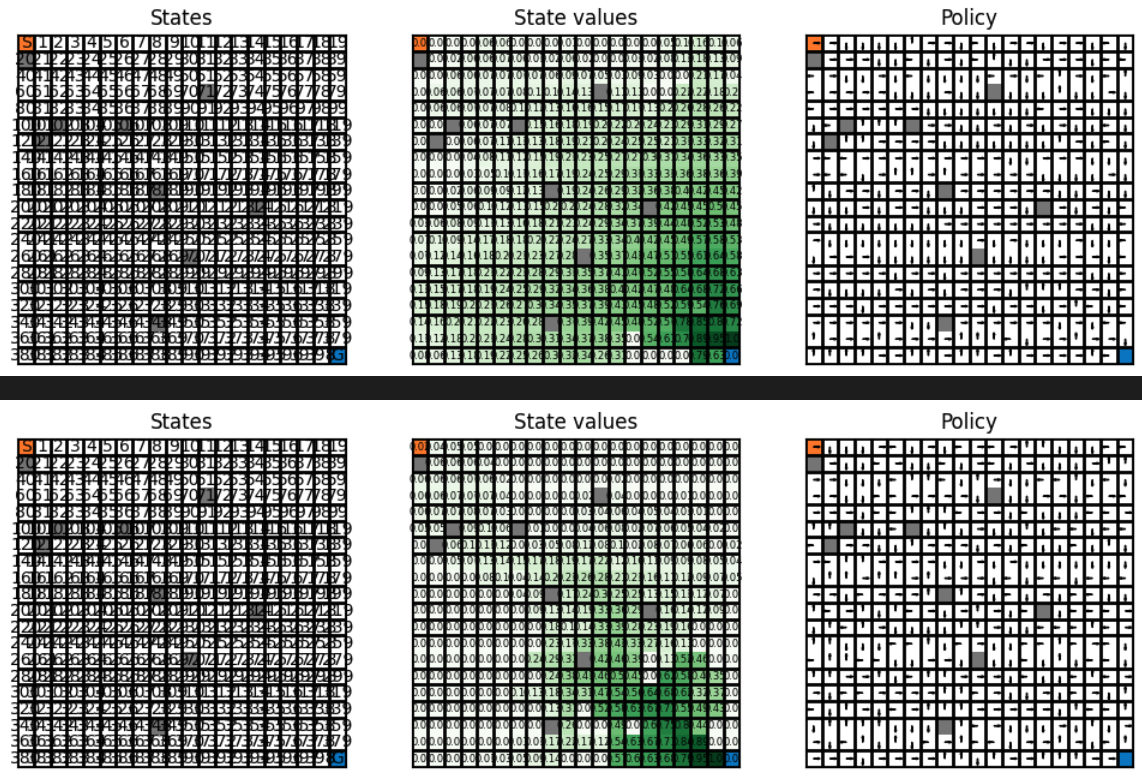
\includegraphics[width=0.8\textwidth]{Assignment2/Images/20x20_50_1.png}
    \caption{State values and policy visualization in the larger 20x20 Gridworld.}
    \label{fig:large_values_policy}
\end{figure}


\noindent In terms of sample efficiency, plots of environment steps per episode demonstrate that Prioritized Sweeping consistently requires fewer real environment interactions than Dyna-Q, particularly after the initial learning episodes. This advantage is further supported by cumulative interaction plots, where Prioritized Sweeping achieves comparable or superior results with fewer cumulative environment steps. Additionally, it can be seen that while they both converge to a similar policy in terms of step count to reach the goal: Prioritised Sweeping converges faster than Dyna-Q. The two prior statements are portrayed in the graphs below, which show the already big difference between the two models on the original settings of the Gridworld (Figure 3), which becomes even bigger if we increase the Gridworld environment to 20x20 (Figure 4).

\begin{figure}[htbp]
  \centering
  \begin{subfigure}[b]{0.48\textwidth}
    \centering
    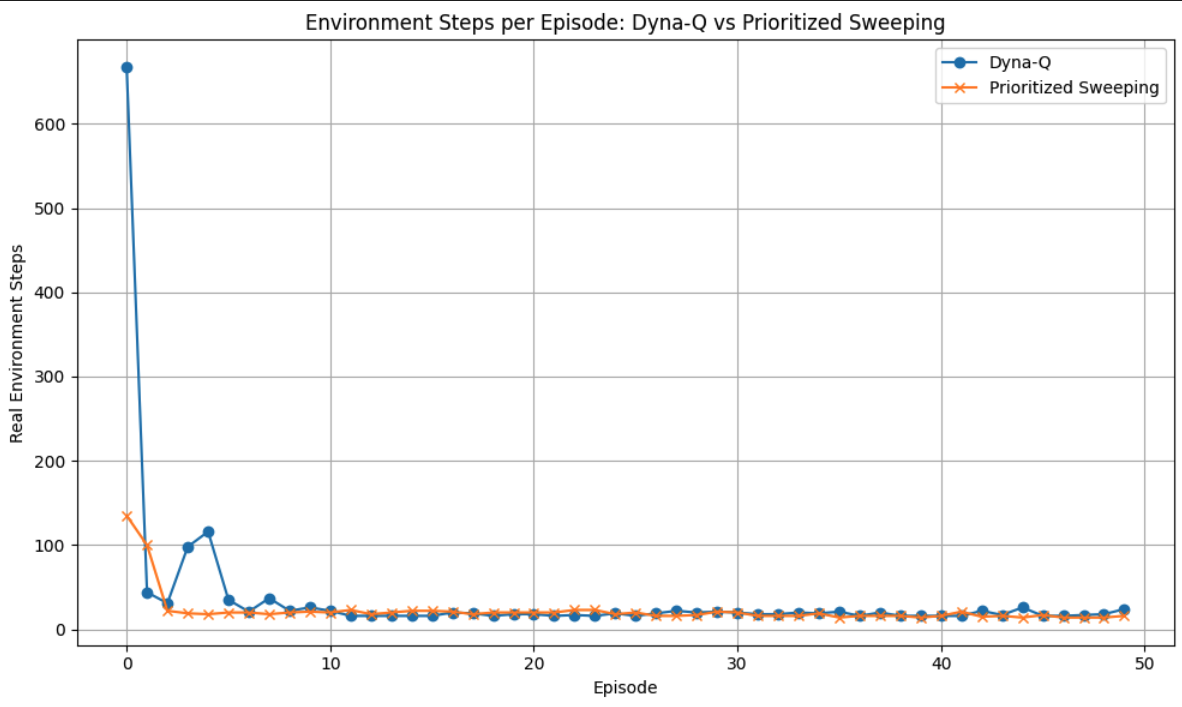
\includegraphics[width=\textwidth]{Assignment2/Images/original_50_2.png}
    \label{fig:original_steps_per_episode}
  \end{subfigure}
  \hfill
  \begin{subfigure}[b]{0.48\textwidth}
    \centering
    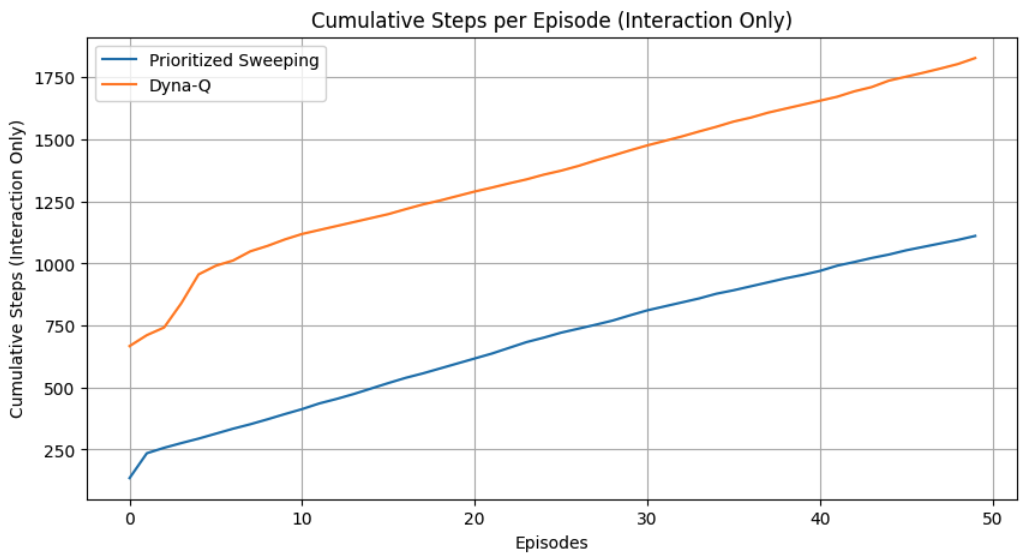
\includegraphics[width=\textwidth]{Assignment2/Images/original_50_3.png}
    \label{fig:original_cumulative_steps}
  \end{subfigure}
  \caption{Comparison of Prioritized Sweeping and Dyna-Q in the original 6x9 Gridworld environment.}
  \label{fig:original_side_by_side}
\end{figure}

\begin{figure}[htbp]
  \centering
  \begin{subfigure}[b]{0.48\textwidth}
    \centering
    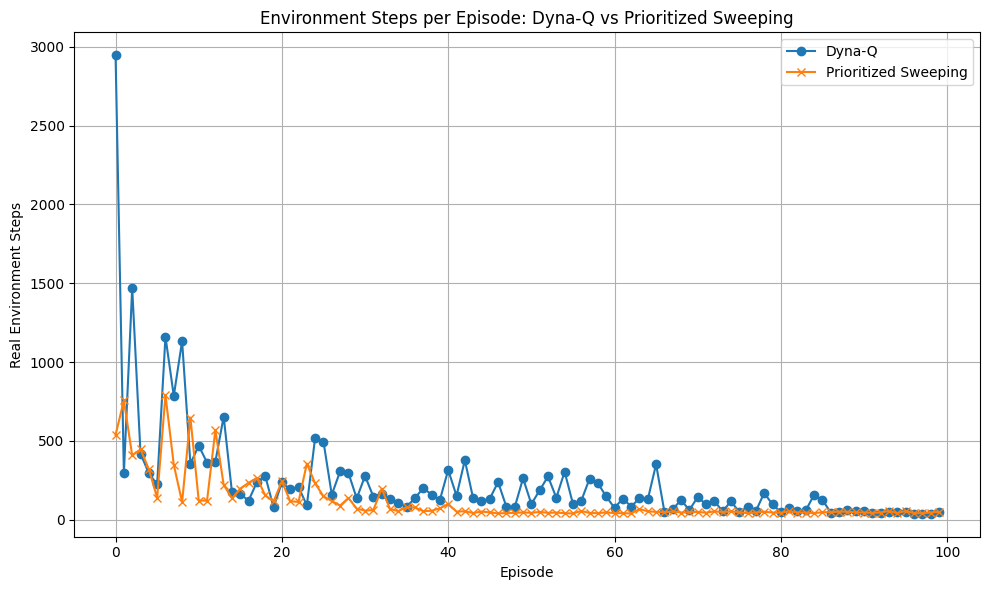
\includegraphics[width=\textwidth]{Assignment2/Images/20x20_2.png}
    \label{fig:large_steps_per_episode}
  \end{subfigure}
  \hfill
  \begin{subfigure}[b]{0.48\textwidth}
    \centering
    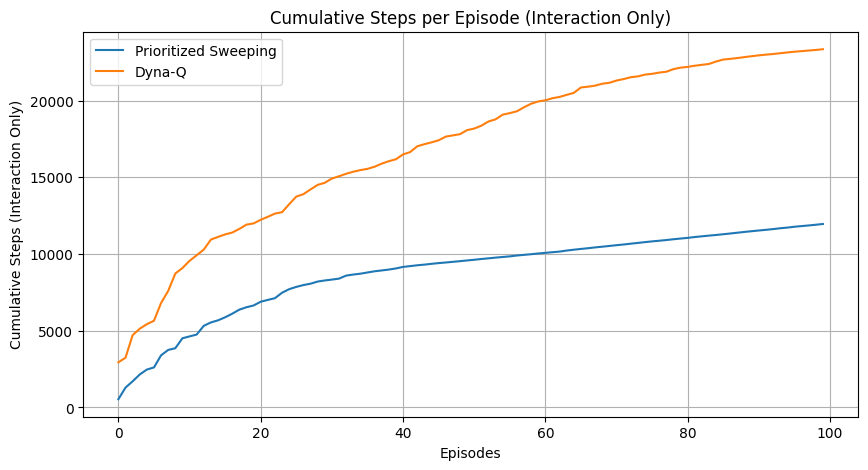
\includegraphics[width=\textwidth]{Assignment2/Images/20x20_3.png}
    \label{fig:large_cumulative_steps}
  \end{subfigure}
  \caption{Performance comparison in a larger 20x20 Gridworld environment, highlighting the scalability advantage of Prioritized Sweeping.}
  \label{fig:large_side_by_side}
\end{figure}


\noindent While Prioritized Sweeping requires more computing power, mainly because it has to keep a priority queue and make targeted updates, it makes up for it by learning faster and producing more accurate value estimates. On the other hand, Dyna-Q is easier to set up and runs more efficiently, but it's generally slower to converge and produces lower-quality policies. That’s why, in settings where interactions with the environment are costly or limited, like in robotics or real-world simulations, Prioritized Sweeping is often the better choice.

\pagebreak

\section{Question}

\section*{Introduction}

In their paper \textit{``Mastering Chess and Shogi by Self-Play with a General Reinforcement Learning Algorithm''}, Silver et al. introduce \textbf{AlphaZero}, a reinforcement learning system that learns to play games like chess, shogi (Japanese chess), and Go at a superhuman level, entirely from scratch. What makes this achievement remarkable is that AlphaZero starts from random play, without any human data, domain-specific knowledge, or expert-crafted rules. It is guided only by the basic rules of each game and learns entirely through self-play. \\

\noindent This work builds on the AlphaGo Zero framework but takes it a step further by applying the same, fully general algorithm to multiple games. The result is a single, unified approach that adapts and excels across very different strategic environments, proving that strong artificial intelligence doesn’t need game-specific programming, it just needs the ability to learn.


\section*{Self-Play and Reinforcement Learning Framework}

AlphaZero relies on a closed loop of self-improvement driven by self-play. It begins with random play and gradually improves by continually training on the data it generates. The algorithm's central components include a deep neural network and Monte Carlo Tree Search (MCTS). The neural network, denoted $f_\theta(s)$, takes a board state $s$ and outputs a policy $\pi(a|s)$, representing the probability distribution over legal moves, and a value $v(s)$ estimating the expected game outcome (win, loss, or draw). \\

\noindent At each turn, AlphaZero uses a version of Monte Carlo Tree Search (MCTS) to look ahead by simulating possible move sequences. These simulations are guided by the neural network’s current understanding of the game. The algorithm selects moves that strike a balance between exploration (trying less-visited paths) and exploitation (choosing moves that seem valuable based on past simulations) (i.e. a balance between low visit count, high prior probability, and high estimated
value). The search produces a refined policy vector $\pi$ over moves and returns an outcome z
indicating the result of the simulation (+1 for win, 0 for draw, -1 for loss). These outcomes
inform the neural network’s learning through stochastic gradient descent.


\section*{Generalization from AlphaGo Zero}

While inspired by AlphaGo Zero, AlphaZero introduces several key differences that make it more general:

\begin{itemize}
    \item \textbf{Draws matter:} AlphaGo Zero optimized a binary win/loss outcome, ignoring draws. AlphaZero models the expected outcome, including draws, critical for chess and shogi.
    \item \textbf{Continuous Learning:} AlphaGo Zero maintained two players: the best previous version and the current version, updating only if the new version surpassed 55\% win rate. AlphaZero uses a single continuously updated network.
    \item \textbf{No Data Augmentation:} AlphaGo Zero used 8-fold symmetry augmentation and board transformations during MCTS. AlphaZero uses no such augmentations or transformations.
    \item \textbf{No Tuning for specific games:} AlphaGo Zero employed Bayesian optimization for hyperparameter tuning. AlphaZero uses the same hyperparameters across all games, only adjusting the Dirichlet noise scale according to the number of legal moves.
\end{itemize}

\section*{Performance and Efficiency}

AlphaZero’s performance highlights the strength of qualitative, rather than brute-force, search. While Stockfish (chess) and Elmo (shogi) search 70 million and 35 million positions per second respectively, AlphaZero only searches 80,000 (chess) and 40,000 (shogi) positions per second. Despite this, it outperforms both, demonstrating that efficient learning can overcome raw computational brute force. \\

\noindent AlphaZero’s approach also differs fundamentally from traditional alpha-beta search. Alpha-beta computes minimax evaluations, often susceptible to propagating errors up the tree. AlphaZero uses MCTS to average evaluations over many simulations, mitigating such risks. Moreover, AlphaZero evaluates positions using deep, non-linear neural networks, enabling richer feature representations than the linear approximators used in most classical engines.

\section*{Neural Architecture and Training Regime}

Each AlphaZero model is trained from scratch for each game, with no transfer learning between them. The policy output is represented as a 3D stack of planes. For example, in chess, it uses an $8 \times 8 \times 73$ tensor encoding 4,672 possible moves. Each MCTS uses 800 simulations per move. The learning rate starts at 0.2 and is reduced (decay) in steps to 0.02, 0.002, and 0.0002 over the course of training. Moves are sampled proportionally to root visit counts. Dirichlet noise is added to the prior policy to encourage exploration.

\section*{Self-Play and Multi-Agent Learning Perspectives}

AlphaZero exemplifies the power of self-play reinforcement learning. It resembles a multi-agent reinforcement learning (MARL) system, where the agent continually plays against and adapts to its most recent version. This creates a dynamically evolving curriculum where the agent faces increasingly challenging opponents, its own previous selves. This self-competition fosters sophisticated emergent strategies without external supervision.

\section*{References}

Silver, D., Hubert, T., Schrittwieser, J., Antonoglou, I., Lai, M., Guez, A., ... & Hassabis, D. (2017). Mastering chess and shogi by self-play with a general reinforcement learning algorithm. arXiv preprint arXiv:1712.01815.

\end{document}
